%% Template para dissertacao/tese na classe UFBAthesis
%% versao 1.0
%% (c) 2005 Paulo G. S. Fonseca
%% (c) 2012 Antonio Terceiro
%% (c) 2014 Christina von Flach
%% www.dcc.ufba.br/~flach/ufbathesis

%% Carrega a classe ufbathesis
%% Opcoes: * Idiomas
%%           pt   - portugues (padrao)
%%           en   - ingles
%%         * Tipo do Texto
%%           bsc  - para monografias de graduacao
%%           msc  - para dissertacoes de mestrado (padrao)
%%           qual - exame de qualificacao de mestrado
%%           prop - exame de qualificacao de doutorado
%%           phd  - para teses de doutorado
%%         * Media
%%           scr  - para versao eletronica (PDF) / consulte o guia do usuario
%%         * Estilo
%%           classic - estilo original a la TAOCP (deprecated) - apesar de deprecated, manter esse.
%%           std     - novo estilo a la CUP (padrao)
%%         * Paginacao
%%           oneside - para impressao em face unica
%%           twoside - para impressao em frente e verso (padrao)

% Atenção: Manter 'classic' na declaracao abaixo:
\documentclass[bsc, en, classic, a4paper]{ufbathesis}

%% Preambulo:
\usepackage[utf8]{inputenc}
\usepackage{graphicx}
\usepackage{lipsum}
\usepackage{hyphenat}
%\usepackage[usenames, dvipsnames, table]{xcolor} %TODO: try to uncomment
\usepackage{booktabs}
\usepackage{pifont}
\usepackage{multirow}
\usepackage{listings} 
\usepackage{colortbl}
\usepackage{xfrac}
%\usepackage[FIGTOPCAP]{subfigure}
\usepackage[printonlyused, withpage]{acronym}

% Custom preamble
\usepackage{cancel}
\usepackage[utf8]{inputenc}
\usepackage{nicefrac}
\usepackage{graphicx}
\usepackage{url}
\usepackage{amsmath}
\usepackage{amsfonts}
%\usepackage{amsthm}
%\usepackage{lineno,hyperref}
\usepackage{algorithm}
\usepackage{algorithmicx}
\usepackage{algpseudocode}
\usepackage{subcaption}
\usepackage{commath}

\newcommand{\etal}{\textit{et~al }}
\newcommand{\refalg}[1]{Algorithm~\ref{alg:#1}}
\newcommand{\reffig}[1]{Figure~\ref{fig:#1}}
\newcommand{\reftab}[1]{Table~\ref{tab:#1}}
\newcommand{\refchap}[1]{chapter~\ref{chap:#1}}
\newcommand{\Refchap}[1]{Chapter~\ref{chap:#1}}
\newcommand{\refsec}[1]{section~\ref{sec:#1}}
\newcommand{\Refsec}[1]{Section~\ref{sec:#1}}
\newcommand{\refsubsec}[1]{subsection~\ref{subsec:#1}}
\newcommand{\Refsubsec}[1]{Subsection~\ref{subsec:#1}}
\newcommand{\procedure}[1]{{\scshape #1}}
\newcommand{\href}[2]{#1} % href completely breaks citations
\newcommand{\vc}[1]{\mathbf{#1}}

% Universidade
\university{Universidade Federal da Bahia}

% Endereco (cidade)
\address{Salvador}

% Instituto ou Centro Academico
\institute{Instituto de Matem\'{a}tica e Estatística}

% Nome da biblioteca - usado na ficha catalografica
\library{Biblioteca Reitor Mac\^{e}do Costa} %TODO: is this correct?

% Programa de pos-graduacao %TODO: is this correct?
\program{Programa de Graduação em Ciência da Computação}

% Area de titulacao
\majorfield{Ci\^{e}ncia da Computa\c{c}\~{a}o}

% Titulo da dissertacao
\title{A deep learning approach to recognize source code authorship}

% Data da defesa
% e.g. \date{19 de fevereiro de 2013}
%TODO: set date
\date{?? de dezembro de 2018}
% e.g. \defenseyear{2013}
\defenseyear{2018}

% Autor
% e.g. \author{Jose da Silva}
\author{Roberto Sales Caldeira}

% Orientador(a)
% Opcao: [f] - para orientador do sexo feminino
% e.g. \adviser[f]{Profa. Dra. Maria Santos}
\adviser{Maurício Pamplona Segundo}

% Orientador(a)
% Opcao: [f] - para orientador do sexo feminino
% e.g. \coadviser{Prof. Dr. Pedro Pedreira}
% Comente se nao ha co-orientador
%\coadviser{Nome Completo do CO-ORIENTADOR}

%% Inicio do documento
\begin{document}

%TODO: change to \frontpage?
\pgcompfrontpage

%% Parte pre-textual
\frontmatter

\presentationpage

%%%%%%%%%%%%%%%%%%%%%%%%%
% Ficha catalografica
%%%%%%%%%%%%%%%%%%%%%%%%%

\authorcitationname{Sales, Roberto} % e.g. Terceiro, Antonio Soares de Azevedo
\advisercitationname{Pamplona, Maurício} % e.g. Chavez, Christina von Flach Garcia
%\coadvisercitationname{Sobrenome, Nome do CO-ORIENTADOR} % e.g. Mendonca, Manoel Gomes de
\catalogtype{Monografia (Graduação)} % e.g. ``Tese (Doutorado)''

\catalogtopics{1. Exact algorithm. 2. Isometric embedding. 3. Maximum norm} % Listar palavras-chave do trabalho para a FICHA CATALOGRAFICA}, por exemplo, ``1. Complexidade Estrutural. 2. Qualidade de Software 3. Engenharia de Software''
\catalogcdd{XXX.XX} % e.g.  XXX.XX (número nesse formato serah dado pela biblioteca)
\catalogcdu{XXX.XX.XXX} % e.g.  XXX.XX.XXX (idem) 
\catalogingsheet

%%%%%%%%%%%%%%%%%%%%%
% Termo de aprovacaoo
%%%%%%%%%%%%%%%%%%%%%

%TODO: set date e banca
\approvalsheet{Salvador, ?? de dezembro de 2018}{
   \comittemember{Prof. Dr. Maurício Pamplona Segundo}{Universidade Federal da Bahia}
   \comittemember{Prof. Dr. Professor 2}{Universidade Federal da Bahia}
   \comittemember{Profa. Dra. Professora 3}{Universidade Federal da Bahia}
   % Para mestrado, apenas 3.
   % \comittemember{Prof. Dr. Professor 4}{Universidade HJKL}
   % \comittemember{Profa. Dra. Professora 5}{Universidade QWERTY}
}

%%%%%%%%%%%%%%%%%%%%%%%%%%%%%%%%%%%%%%%%
% Dedicatoria, Agradecimentos, Epigrafe
%%%%%%%%%%%%%%%%%%%%%%%%%%%%%%%%%%%%%%%%

%TODO: write dedicatory
% Comente para ocultar
\begin{dedicatory}
DIGITE A DEDICATORIA AQUI
\end{dedicatory}

% Agradecimentos
% Se preferir, crie um arquivo `a parte e o inclua via \include{}
\acknowledgements
%TODO: write acknowledgements
DIGITE OS AGRADECIMENTOS AQUI

% Epigrafe
%TODO: write epigraph
\begin{epigraph}[NOTA]{AUTOR}
DIGITE AQUI A CITACAO
\end{epigraph}

%%%%%%%%%%%%%%%%%%%%%
% Resumo em Portugues
%%%%%%%%%%%%%%%%%%%%%

%TODO: write abstract in Portuguese
\resumo
COLOQUE O RESUMO. Se preferir, crie um arquivo separado e o inclua via comando include.

Para evitar problemas de formato neste template (de uso geral), usamos acentua\c{c}\~{a}o mostrada abaixo. 

\begin{verbatim} 
\c{c} \~{a} \'{a} \^{e} \'{\i}
\end{verbatim} 

N\~{a}o precisa fazer dessa forma, caso use pacotes adequados (latin1, etc.).

%TODO: write keywords in Portuguese
% Palavras-chave do resumo em Portugues
\begin{keywords}
PALAVRAS-CHAVE.
\end{keywords}

%%%%%%%%%%%%%%%%%%%
% Resumo em Ingles
%%%%%%%%%%%%%%%%%%%

\abstract
Source code authorship identification is the task of deciding who is the author of a program given its source code. This is usually based on the analysis of previously collected samples from a set of candidate authors. There are several use cases for such a method, including attribution and detection of malicious codes, copyright infringement incident resolution, plagiarism detection, etc. As with texts in natural language, there are many distinguishing features in a piece code, like variable names, indentation style, etc. Some of these features are part of the coding style of a programmer. In this work, we investigate authorship attribution of C++ source codes based on the coding style of the authors. We also propose an end-to-end deep learning method for deciding if two source codes are from the same author, even if the involved authors are unknown to the system.
% Palavras-chave do resumo em Ingles
\begin{keywords}
software forensics, authorship identification, plagiarism detection
\end{keywords}

%%%%%%%%%%%%%%%%%%%
% Sumario / Indice
%%%%%%%%%%%%%%%%%%%

% Comente para ocultar
\tableofcontents

% Lista de figuras
% Comente para ocultar
\listoffigures

% Lista de tabelas
% Comente para ocultar
%\listoftables


\iffalse
\chapter*{Lista de Siglas}

% Sintaxe da lista de acordo com a documentação do pacote `acronym'
% documentação: http://mirror.unl.edu/ctan/macros/latex/contrib/acronym/acronym.pdf
\begin{acronym}[PGCOMP]
    \acro{PGCOMP}{Programa de Pós-Graduação em Ciência da Computação}
    \acro{CNPq}{Conselho Nacional de Desenvolvimento Centífico e Tecnológico}
\end{acronym}
\fi

%% Parte textual
\mainmatter

%\input{content-sample}
\xchapter{Introduction}{}

Programmers often have to choose between tabs and spaces, between \texttt{while} loops and \texttt{for} loops, between positioning the open bracket in the next line or in the current line, etc. These are choices that can be regarded as their coding styles. Are these choices distinguishable features? In this chapter we will discuss what is style-based source code authorship identification, what challenges it poses, what has been done and what it is useful for. We will also introduce our contributions on the subject.

\section{Biometry and Coding Style}

\section{Motivation}

Throughout this work, we mainly consider the task of an investigator interested in deciding whether two anonymous pieces of code were authored by the same programmer or not. The actual authors of these pieces of code may be unknown to the investigator. Also, these codes may aim to solve different problems, therefore the investigator intends to distinguish them solely based on stylistic features of such pieces.

We also consider easier scenarios where the set of possible authors are known to the investigator and labeled samples from this set are available. % TODO: link to section where these are formulated

We approach these problems from a deep learning perspective, training a deep neural model that can be subsequently used to resolve authorship of source codes and applying it to the different scenarios an investigator can face.

\section{Applications}

Resolving source code authorship has a few real-world applications both in industry and academy. Although we haven't directly studied those, in this section we briefly describe them a few of them. In section (...) we also describe how the experimental formulations we propose in section (...) are related to each of them.

\subsection{Plagiarism Detection}

% alguma referencia q reforce esse paragrafo?
Plagiarism can be generally defined as the unauthorized re-use of the work of another individual. Source code plagiarism is a widespread problem in academic institutions. Checking for plagiarism manually is time-consuming and not extremely effective, becoming impractical as the size of the codebase increases.

Although automatic source code plagiarism detection is a recurring and well-studied problem \cite{plag_survey}, the approaches consolidated by widely used tools such as MOSS \cite{moss}, Sherlock and JPlag \cite{jplag} are mainly based on code similarity metrics which are greatly correlated to the task the code was written to solve.% refer to these tools

For example, let's consider the specific case of \textit{ghostwriting}, where the code the individual claims to be of his authorship was neither written by him nor copied from a colleague, but was actually written by another person (a former student, for example).  It may not be possible to compare the suspicious code with another code by the same author, since the ghostwriter may actually be unknown. On the other hand, if pieces of code of the accused party are available, it's possible to determine if his coding style matches the coding style present in the suspicious code.

Also, an analyst may strongly suspect that a piece of code a programmer claims to be of his authorship is actually not, but have no clue of who the actual author might be. This can be modeled as a binary classification problem where positive samples are other pieces of code of the same author and negative samples are pieces from unrelated programmers. We propose another approach to this problem in (...).

\subsection{Copyright Infringement}

Software forensics is the science of examining source code and binary code in order to identify, preserve, analyze and present facts and opinions about pieces of software. Although it can also be used in civil proceedings, it's most often associated with the investigation of a wide variety of computer crimes, one of which is copyright infringement.

Code correlation analysis plays an important role at copyright disputes. In this case, an analyst has labeled codes from the involved parties and the task of determining if there was infringement or not.

\subsection{Cyber Attack Identification}

Cyber attack identification is a powerful application of software forensics in cyber security. Files left behind by an intruder during a cyber attack may have just enough information for an analyst to identify who the intruder is or to relate such an attack to a previous incident. Therefore, comparing the coding style of the attacker to those of authors of previous attacks and authors of public code repositories is of great interest to the analyst.

\subsection{Exposing Anonymous Programmers}

Although there are many helpful applications of source code authorship identification, systems capable of de-anonymizing programmers pose a threat to those who want to remain anonymous, in special for anonymous open source contributors. In particular, \cite{gitblame} shows how effectively modern methods can identify authorship of small pieces of code from GitHub repositories .There may be good reasons for a programmer to be anonymous, like working in a software a hostile government doesn't like. 

An example of a famous open source anonymous programmer is Bitcoin's creator, Satoshi Nakamoto. For example, if we had a set of labeled codes from programmers that are likely to be Nakamoto, we could try to match their coding style to the early versions of Bitcoin, of course assuming that Nakamoto didn't try to obfuscate his own coding style.

\section{Challenges}

\section{Contribution}
\xchapter{Methodology}{}

In this chapter, we present formulations to the many variants of the source code attribution problem in Section \ref{sec:formulations}, we describe how the Codeforces dataset was assembled in Section \ref{sec:dataset} and present a top-down approach to how the end-to-end model was developed in section \ref{sec:framework}.

\section{Problem Formulation}\label{sec:formulations}
\section{Datasets}\label{sec:dataset}

The first step to develop an effective deep learning model is to gather enough training data. In this work, we decided to work with C++ source codes written in a laboratory environment -- we assume the whole code is written by the author under no external style enforcement such as a style guide.

\subsection{Google Code Jam}

Although there are many public C++ laboratory datasets, the Google Code Jam\footnote{\url{https://codingcompetitions.withgoogle.com/codejam}} dataset \cite{caliskan_2015} is probably the biggest of them all. Samples from this dataset are collected from previous editions of Google Code Jam, an annual programming competition held by Google. In this competition, participants are given algorithmic tasks to be solved in a limited amount of time. As such, it's very likely that code written by a participant manifests his own coding style.

Google Code Jam holds nearly 10 rounds every year. Most of these rounds are eliminatory. Thus, the availability of samples from less experienced participants is expected to be low. If we want to build a balanced training set not biased by the way experienced participants code, we are limited by the small amount of code less experienced participants wrote.

Although this dataset was not extensively used throughout the development phase, it was a reference for the Codeforces dataset introduced in Section \ref{sec:codeforces}.

\subsection{Codeforces}\label{sec:codeforces}

Codeforces\footnote{\url{http://codeforces.com}} is a website specialized in holding online programming contests. Contest format is similar to Google Code Jam's, but they are not eliminatory. Thus, we are able to find a lot of samples from both non-experienced and experienced users.

We wrote a Python script that receives target constraints for the dataset and scrapes Codeforces for samples. Using this script, we assembled a balanced dataset with more than 30,000 samples from nearly 2,000 authors, meaning that we have around 15 samples per author. This dataset was packaged and made public\footnote{link-pro-dataset}.
% TODO: more details on filters
% TODO: add link to dataset

\section{Source Code Embedding Model}\label{sec:framework}

In this section, we propose a deep learning model that embeds source codes, from their string representations, into a denser latent space. In Section \ref{sec:descriptor}, we describe what is a style descriptor. In Section \ref{sec:models}, we describe network architectures used in our work. In Section \ref{sec:optimization}, we describe how our embedding network was trained to generate meaningful descriptors.

\begin{figure}[ht]
	\centering
	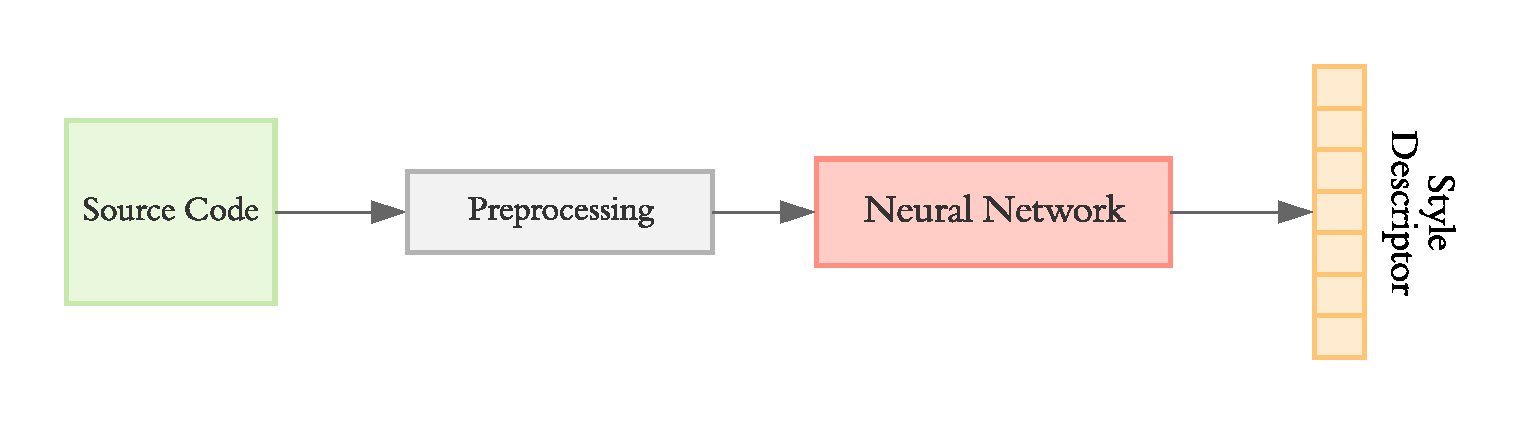
\includegraphics[width=\linewidth]{imgs/pipeline.pdf}
	\caption{Overview of style descriptor generation pipeline.}
	\label{fig:overall}
\end{figure}
% TODO: se referir a essa figura em algum lugar

\subsection{Coding Style Descriptor}\label{sec:descriptor}

The performance of machine learning methods is heavily affected by the choice of data representation. Thus, much of the effort of the machine learning community has been put into developing algorithms that transform otherwise unmanageable data into representations that can be effectively used by learning methods \cite{representation_learning}.

A Coding Style Descriptor (hereon referred simply as \textit{style descriptor}) is a $d$-dimensional representation of a source code in a latent space. A latent space is a space where representations of similar objects lie close to each other. Therefore, the latent space of style descriptors should capture stylistic similarities of source codes. Ideally, style descriptors should encode everything a machine learning model needs to solve the problems posed in Section \ref{sec:formulations}. Thus, we can build simpler classifiers for these problems if we can provide a good embedding function $f(x) \in \mathbb{R}^d$, which maps source codes to $d$-dimensional descriptors.

% TODO: add references to embedding being succesfully applied in conjunction with deep learning

Deep feed-forward networks are a natural approach to representation learning. In the remainder of this chapter, we will mainly study deep learning embedding techniques and apply them to our problem.

\subsection{Preprocessing}\label{sec:preprocessing}

Using Tensorflow static graph, it is not possible to support arbitrary input sizes in a batch. Therefore, we must crop our source code to a maximum line length $M$ and a maximum number of lines $L$, converting it to a $L \times M$ char matrix. The positions that do not correspond to a char in the source code are masked out both during inference and during optimization. For the models we propose, we chose values of $M$ and $L$ that incurred the best improvement while keeping the training time affordable.0

\subsection{Model based on Convolutional Networs}

\subparagraph*{Network Architecture}

\subsection{Model based on Long Short-Term Memory Networks}

Recurrent neural networks (RNNs) were introduced to solve the lack of persistence of feed-forward networks. They are networks with loops in them. They are fed from an external input -- a sequence -- and from their own output (Fig \ref{fig:rnn:generic}). Although generic RNNs are powerful and in theory are capable of learning any kind of sequence dependency, in practice they struggle to handle those that are long-term. The problems of training RNNs with gradient descent were studied by \citeonline{rnn_sgd}.

\begin{figure}[ht]
	\centering
	\begin{subfigure}[t]{0.25\textwidth}
		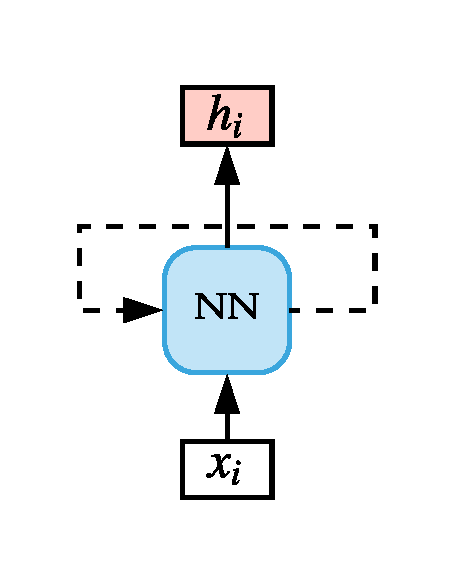
\includegraphics[width=\linewidth]{imgs/rnn.pdf}
		\subcaption{A generic RNN}\label{fig:rnn:generic}
	\end{subfigure}%
	\begin{subfigure}[t]{0.60\textwidth}
		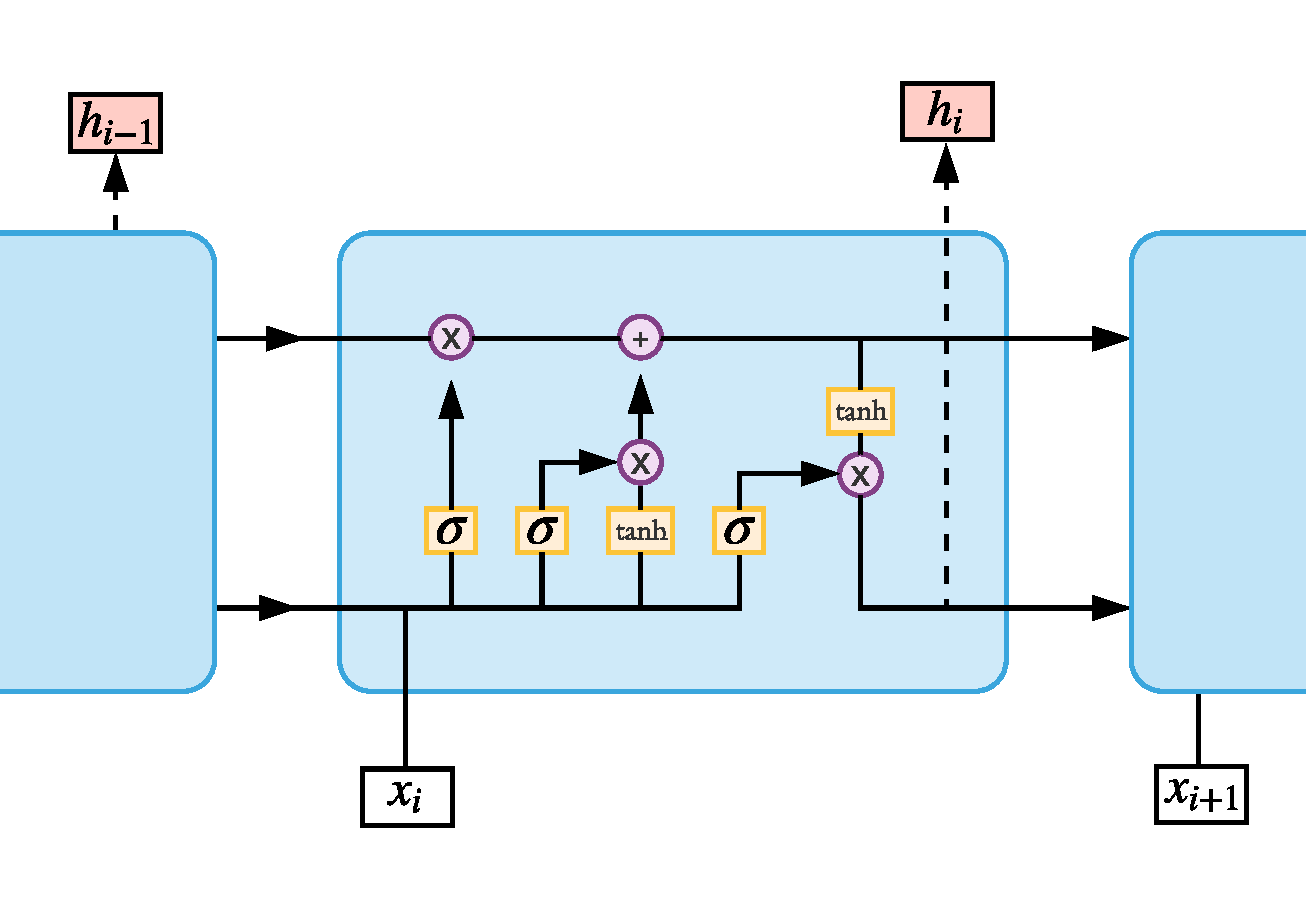
\includegraphics[width=\linewidth]{imgs/lstm_cell.pdf}
		\subcaption{An LSTM cell}\label{fig:rnn:lstm}
	\end{subfigure}%
	\caption{A quick view on the internals of an LSTM.}
	\label{fig:rnn}
\end{figure}

\subparagraph*{Network Architecture}

Our proposed architecture can be split in three parts: the char embedding layer, the line descriptor module (Fig. \ref{fig:lstm_architecture:a}) and the style descriptor module (Fig. \ref{fig:lstm_architecture:b}).

\begin{figure}[htbp]
	\centering
	\begin{subfigure}[t]{\textwidth}
		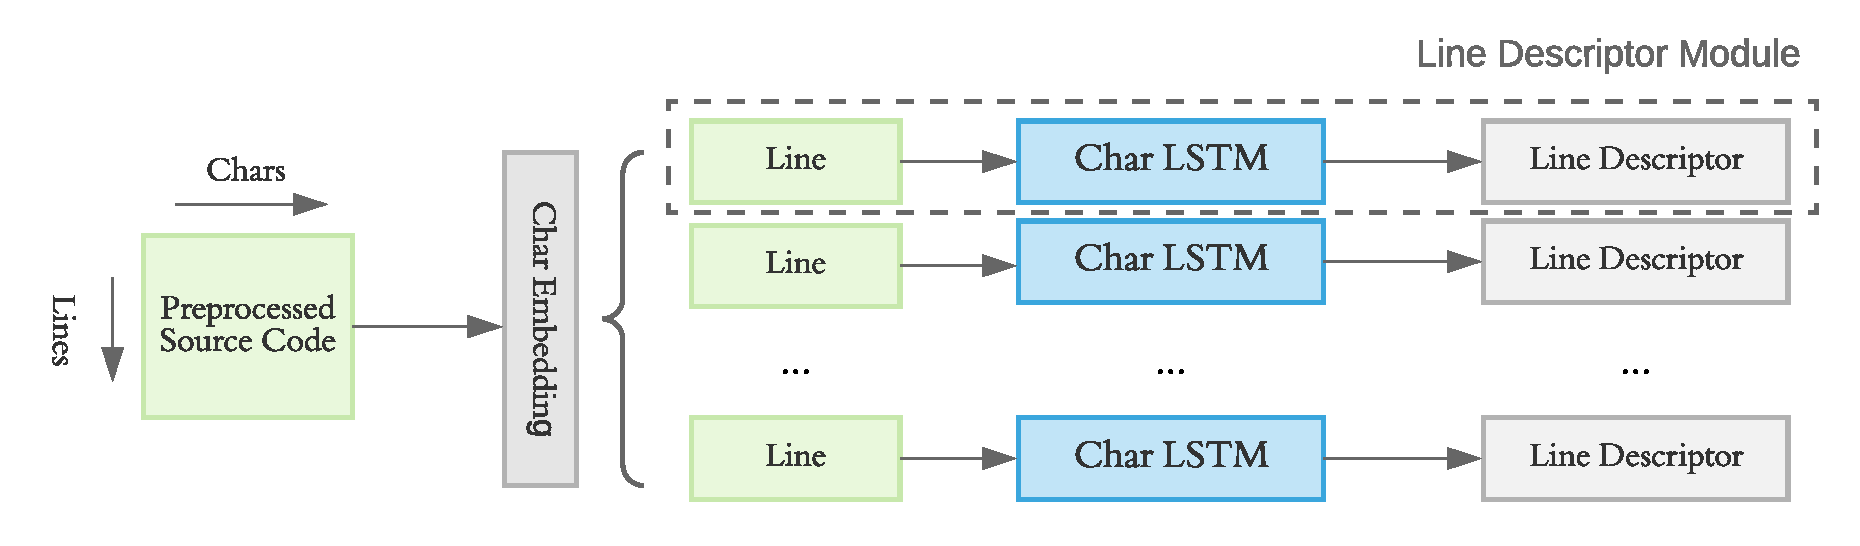
\includegraphics[width=\linewidth]{imgs/lstm_char_level.pdf}
		\subcaption{Char embedding layer and line descriptor module}\label{fig:lstm_architecture:a}
	\end{subfigure}%
	\\
	\begin{subfigure}[t]{\textwidth}
		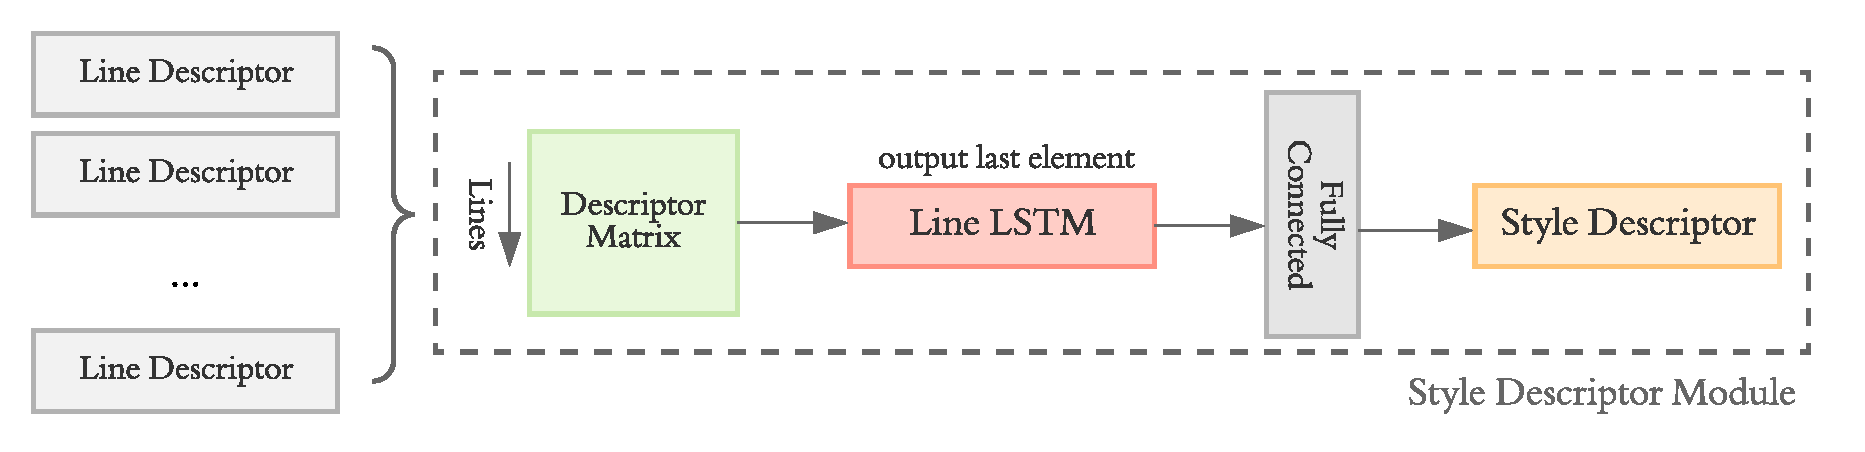
\includegraphics[width=\linewidth]{imgs/lstm_line_level.pdf}
		\subcaption{Style descriptor module}\label{fig:lstm_architecture:b}
	\end{subfigure}%
	\caption{The architecture of the LSTM-based model.}
	\label{fig:lstm_architecture}
\end{figure}

\subparagraph*{Char Embedding Layer}

Neural networks can't handle discrete types -- like chars -- naturally. As such, we need to map the alphabet $\Sigma$ of source codes to real-valued vectors. We could simply convert each char to a $|\Sigma|$-dimensional one-hot vector. As opposed to arbitrarily defining a mapping, we can also let the network learn it. 

The char embedding layer is responsible for learning an embedding $f_c(x) \in \mathbb{R}^{d_c}$ that maps chars to $d_c$-dimensional vectors. Thus, each char in the source code is converted to a real-valued vector. Hereon, we will simply refer to char embeddings as chars.
% TODO: add referencia pro embedding do keras

\subparagraph*{Line Descriptor Module} 

This module is responsible for learning an embedding $f_l(x) \in \mathbb{R}^{d_l}$ that maps lines of code to $d_l$-dimensional descriptors. Each line of the source code is fed -- char by char -- to the same char-level bidirectional LSTM.

\subparagraph*{Style Descriptor Module}

The line descriptors generated by the line descriptor module are stacked back into a descriptor matrix. This module is responsible for learning an embedding $f_s(x) \in \mathbb{R}^d$ that maps descriptor matrices to $d$-dimensional style descriptors. Thus, the whole descriptor matrix is fed -- line by line -- to a line-level bidirectional LSTM, passed through a fully-connected layer and normalized to lie on the $d$-sphere. The resulting descriptor is the desired style descriptor.

We believe this architecture encourages the network to learn in a divide-and-conquer manner, by learning the individual features of each line and how to combine them into a single descriptor. The hyperparameter values chosen through the validation phase are given in Table \ref{tab:lstm_hyper}.

% TODO: regenerate this table
\begin{table}[htbp]
	\centering
	\begin{tabular}{c|l}
		\hline
		\textbf{Parameter}           & \multicolumn{1}{c}{\textbf{Value}} \\ \hline
		maximum line length   & (...)                            \\ \hline
		maximum number of lines   & (...)                            \\ \hline
		$d_c$, char embedding size   & (...)                            \\ \hline
		$d_l$, line descriptor size  & (...)                            \\ \hline
		$d$, style descriptor size & (...)                            \\ \hline
		char-level LSTM hidden units & (...)                            \\ \hline
		line-level LSTM hidden units & (...)                            \\ \hline
		fully-connected layer units  & (...)                            \\ \hline
	\end{tabular}
	\caption{Values for the hyperparameters of the LSTM-based model.}
	\label{tab:lstm_hyper}
\end{table}

\subsection{Optimization}\label{sec:optimization}
%TODO: optimization preamble

\subsubsection{Softmax Cross-Entropy Loss}\label{sec:softmax}

The softmax function is commonly used in multi-class classification problems. In a $d$-class scenario, let $f(x) \in \mathbb{R}^d$ be the output of our neural network for a sample $x$. ...

\begin{equation}
q(i) = \frac{e^{f(x)_i}}{\sum_j e^{f(x)_j}} \,.
\end{equation}

$q(i)$ assume values ranging from 0 to 1, and $\sum_i a_i = 1$. Therefore, we can reinterpret $q(i)$ as the estimation of probability the sample $x$ belongs to class $i$. The softmax cross-entropy loss is given as

\begin{equation}
\mathcal{L} = -\sum_{i=1}^d p(x, i) \log q(i) \,,
\end{equation}

where $p(x, i)$ is the actual probability the sample $x$ is from class $i$ (usually a one-hot vector). Thus, by minimizing $\mathcal{L}$, we minimize the cross-entropy between the probability distribution $p$ and an estimated distribution $q$.

Although softmax cross-entropy loss is a very powerful tool, it does not naturally account for the fact that the number of classes may be unknown. Although there are techniques to apply softmax in these scenarios \cite{softmax_trick1,softmax_trick2}, there are other optimization methods designed for such cases. Therefore, we restrict ourselves to use this method only when the number of classes is known.

\subsubsection{Triplet Loss}\label{sec:triplet}

\citeonline{facenet} introduced triplet loss for training embedding networks. In their work, the loss function is used in conjunction with a novel triplet mining algorithm to train an embedding network that maps images to descriptors. These descriptors are then used to solve face recognition. Triplet loss works in scenarios where the number of classes is unknown. As such, it is well-suited for deciding if two pieces of code are of the same person, even if they are unknown to the system.

The embedding is represented by $f(x) \in \mathbb{R}^d$. Additionally, we constrain this embedding to the boundary of a unit $d$-sphere, \textit{i.e.} $\norm{f(x)}_2 = 1$.

Let $a, p, n$ (stand for anchor, positive and negative, respectively) be a triplet from the training set such that $a$ and $p$ have the same label (positive pair), but $a$ and $n$ have different labels (negative pair). Also, let $\mathcal{T}$ be the set of all possible said triplets. Then, triplet loss is defined as

\begin{equation}\label{eq:triplet}
\mathcal{L} = \sum_{(a, p, n) \in \mathcal{T}} %
%\Bigl[\ \norm{f(a) - f(p)}_2 - \norm{f(a) - f(n)}_2 + \alpha \ \Bigr] _+\,,
\max\Bigl(\ \norm{f(a) - f(p)}_2 - \norm{f(a) - f(n)}_2 + \alpha,\ 0\Bigr)\,,
\end{equation}

where $\alpha$ is a margin that is enforced between positive and negative pairs. If $\mathcal{L} = 0$, then for every triplet $(a, p, n) \in T$, it must be true that

\begin{equation}\label{eq:triplet_condition}
\norm{f(a) - f(p)}_2 + \alpha \leq \norm{f(a) - f(n)}_2 \,.
\end{equation}

When Eq. \ref{eq:triplet_condition} is fulfilled, the negative pair of a triplet will be at least as far as the positive pair plus a margin $\alpha$. Thus, by minimizing $\mathcal{L}$, we push the distance of positive pairs towards zero as we push the distance of negative pairs to be greater than the correspondent positive's by $\alpha$. The advantage of this formulation is that, even though all training samples of the same class will form a cluster, they are not required to collapse to a single point. Fig. \ref{fig:triplet} shows a hypothetical scenario of optimization.

Generating all triplets from $\mathcal{T}$ would consider many triplets that easily satistfy Eq. \ref{eq:triplet_condition}. This would cause the training to converge slowly, since those triplets would still be fed to the network, but would not contribute to loss minimization. Therefore, it is crucial to select triplets that do not satisfy this condition to keep improving the model. These are called \textit{hard} triplets.

% TODO: regenerate these pictures with correct casing and alpha
\begin{figure}[ht]
	\centering
	\begin{subfigure}[t]{0.25\textwidth}
		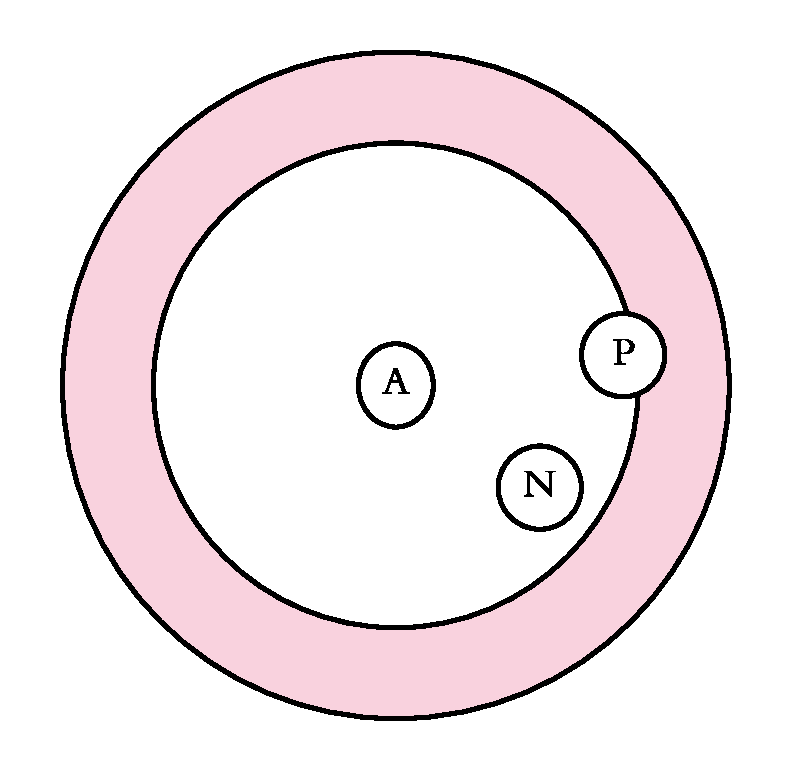
\includegraphics[width=\linewidth]{imgs/triplet_loss_before.pdf}
		\subcaption{}\label{fig:triplet:a}
	\end{subfigure}%
	\hspace{1cm}%
	\begin{subfigure}[t]{0.25\textwidth}
		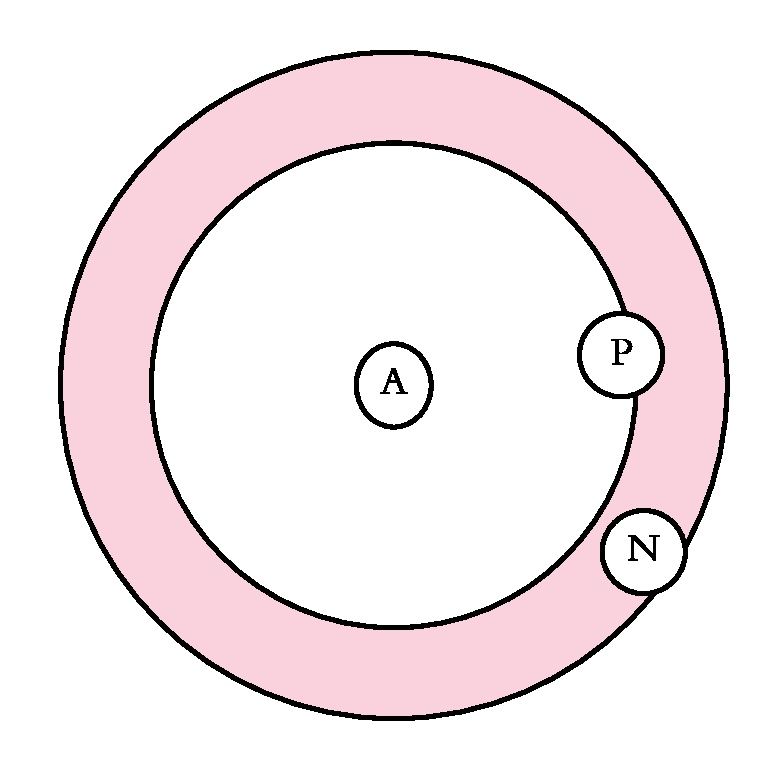
\includegraphics[width=\linewidth]{imgs/triplet_loss_during.pdf}
		\subcaption{}\label{fig:triplet:b}
	\end{subfigure}%
	\hspace{1cm}%
	\begin{subfigure}[t]{0.25\textwidth}
		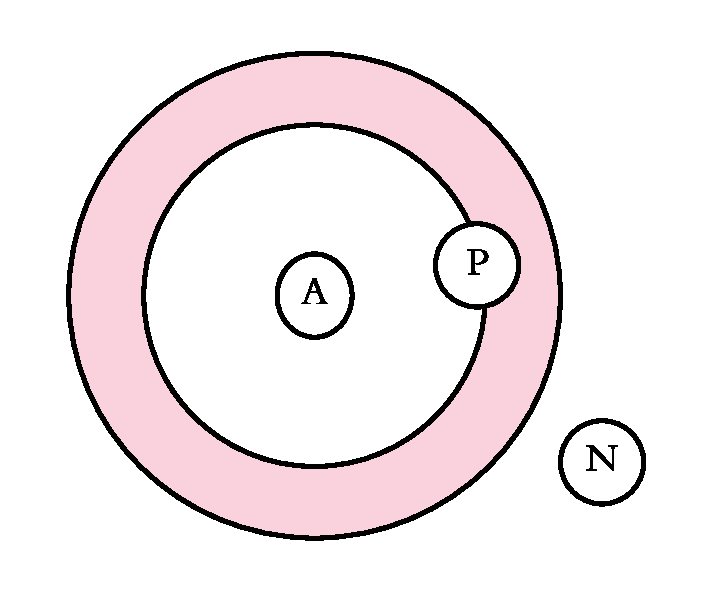
\includegraphics[width=\linewidth]{imgs/triplet_loss_after.pdf}
		\subcaption{}\label{fig:triplet:c}
	\end{subfigure}%
	\caption{The region in red represents the margin area beyond $p$ with diameter $\alpha$. Before loss optimization (\subref{fig:triplet:a}), the negative pair is closer than the positive. During loss optimization (\subref{fig:triplet:b}), the negative pair is pushed further than the positive, but $n$ is still in the margin area. After loss optimization (\subref{fig:triplet:c}), the positive pair is finally closer and $n$ is beyond the margin.}
	\label{fig:triplet}
\end{figure}

\subparagraph*{Online Semi-Hard Triplet Mining} One way to select hard triplets from the training set is to consider every sample as the anchor $a$. Then, select such $p$ that minimizes $\norm{f(a) - f(n)}_2$ and such $n$ that maximizes $\norm{f(a) - f(n)}_2$. This does not scale with the size of the training set. Moreover, it can cause outliers to dominate the selection process. 

\citeauthoronline{facenet} suggested the online semi-hard triplet mining method to tackle both problems. Instead of picking hard triplets from the whole training set, we pick them from the mini-batch. Also, their work suggests that prioritizing triplets such that negatives lie in the margin area (Fig. \ref{fig:triplet:b}) helps avoiding local minima early in the training. Such triplets are called \textit{semi-hard}.

Although in Chapter (...) we use softmax cross-entropy loss for comparison purposes, we mostly worked with triplet loss.  Therefore, our main optimization flow is pictured in Fig. \ref{fig:triplet_overall}.

\begin{figure}[hbpt]
	\centering
	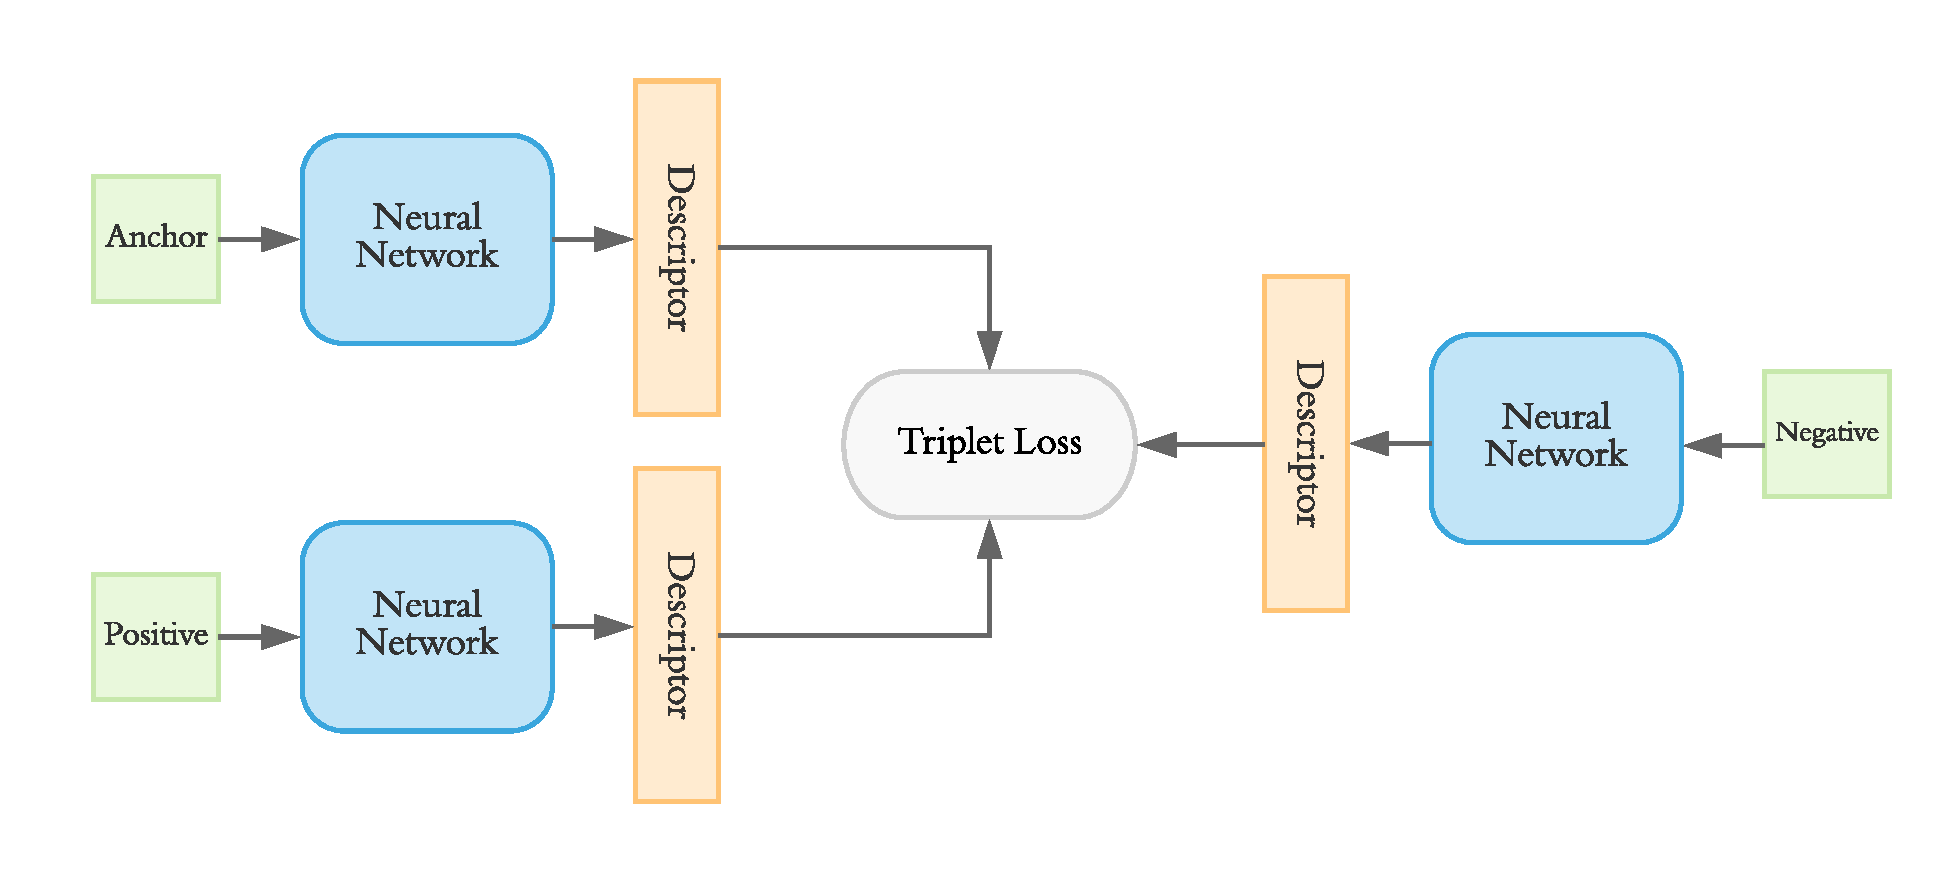
\includegraphics[width=\linewidth]{imgs/triplet_loss_architecture.pdf}
	\caption{Overview of style descriptor generation pipeline.}
	\label{fig:triplet_overall}
\end{figure}
\xchapter{Evaluation}{}\label{chap:evaluation}

In this chapter, we evaluate our model by solving two variations of the source code attribution problem. In Section \ref{sec:validation}, we describe how we selected the parameters of our model. In Section \ref{sec:matching}, we solve the authorship matching problem suggested in Chapter \ref{chap:methodology}. In Section \ref{sec:one_to_many}, we solve a closed-world identification problem.

\section{Training and Selection}\label{sec:validation}

We trained and validated the proposed model with Tensorflow. We picked the training samples from a balanced dataset with 20,000 C++ examples from 1,000 authors. A validation set was built from another 3,200 samples from 400 authors. No author from the training set was present on the validation set. All the samples were extracted from the Codeforces dataset.

Although programming competitions resemble laboratory conditions, it is common for participants to code on top of a pre-written file, usually called \textit{template}. Although the constructions present on a template file are usually written by the author himself, they are not always used by the piece of code actually written during the competition. Therefore, it is interesting to analyze how classifiers perform when such constructions are stripped out of the code. For that end, we used \textit{clang}\footnote{link-do-clang} to remove unused pieces of code from a C++ program. Moreover, we also removed macros, a construction heavily present in templates of competitive programmers. Therefore, we built two versions of each dataset: one composed of raw source codes and other composed of codes processed by \textit{clang}.

We optimized the model parameters with \textit{RMSprop} (...) for a maximum of 50 epochs, or until the evaluated equal error rate (EER) of the model on the validation set had no improvement for 5 epochs. The version that yielded the highest EER was taken as the final model. During this process, we carefully tuned its hyperparameters.

Finally, we trained two different models with such hyperparameters: one on the raw version of the dataset and other on the \textit{clang} processed version.

\section{Matching Two Unknown Source Codes}\label{sec:matching}

\begin{figure}[ht]
	\centering
	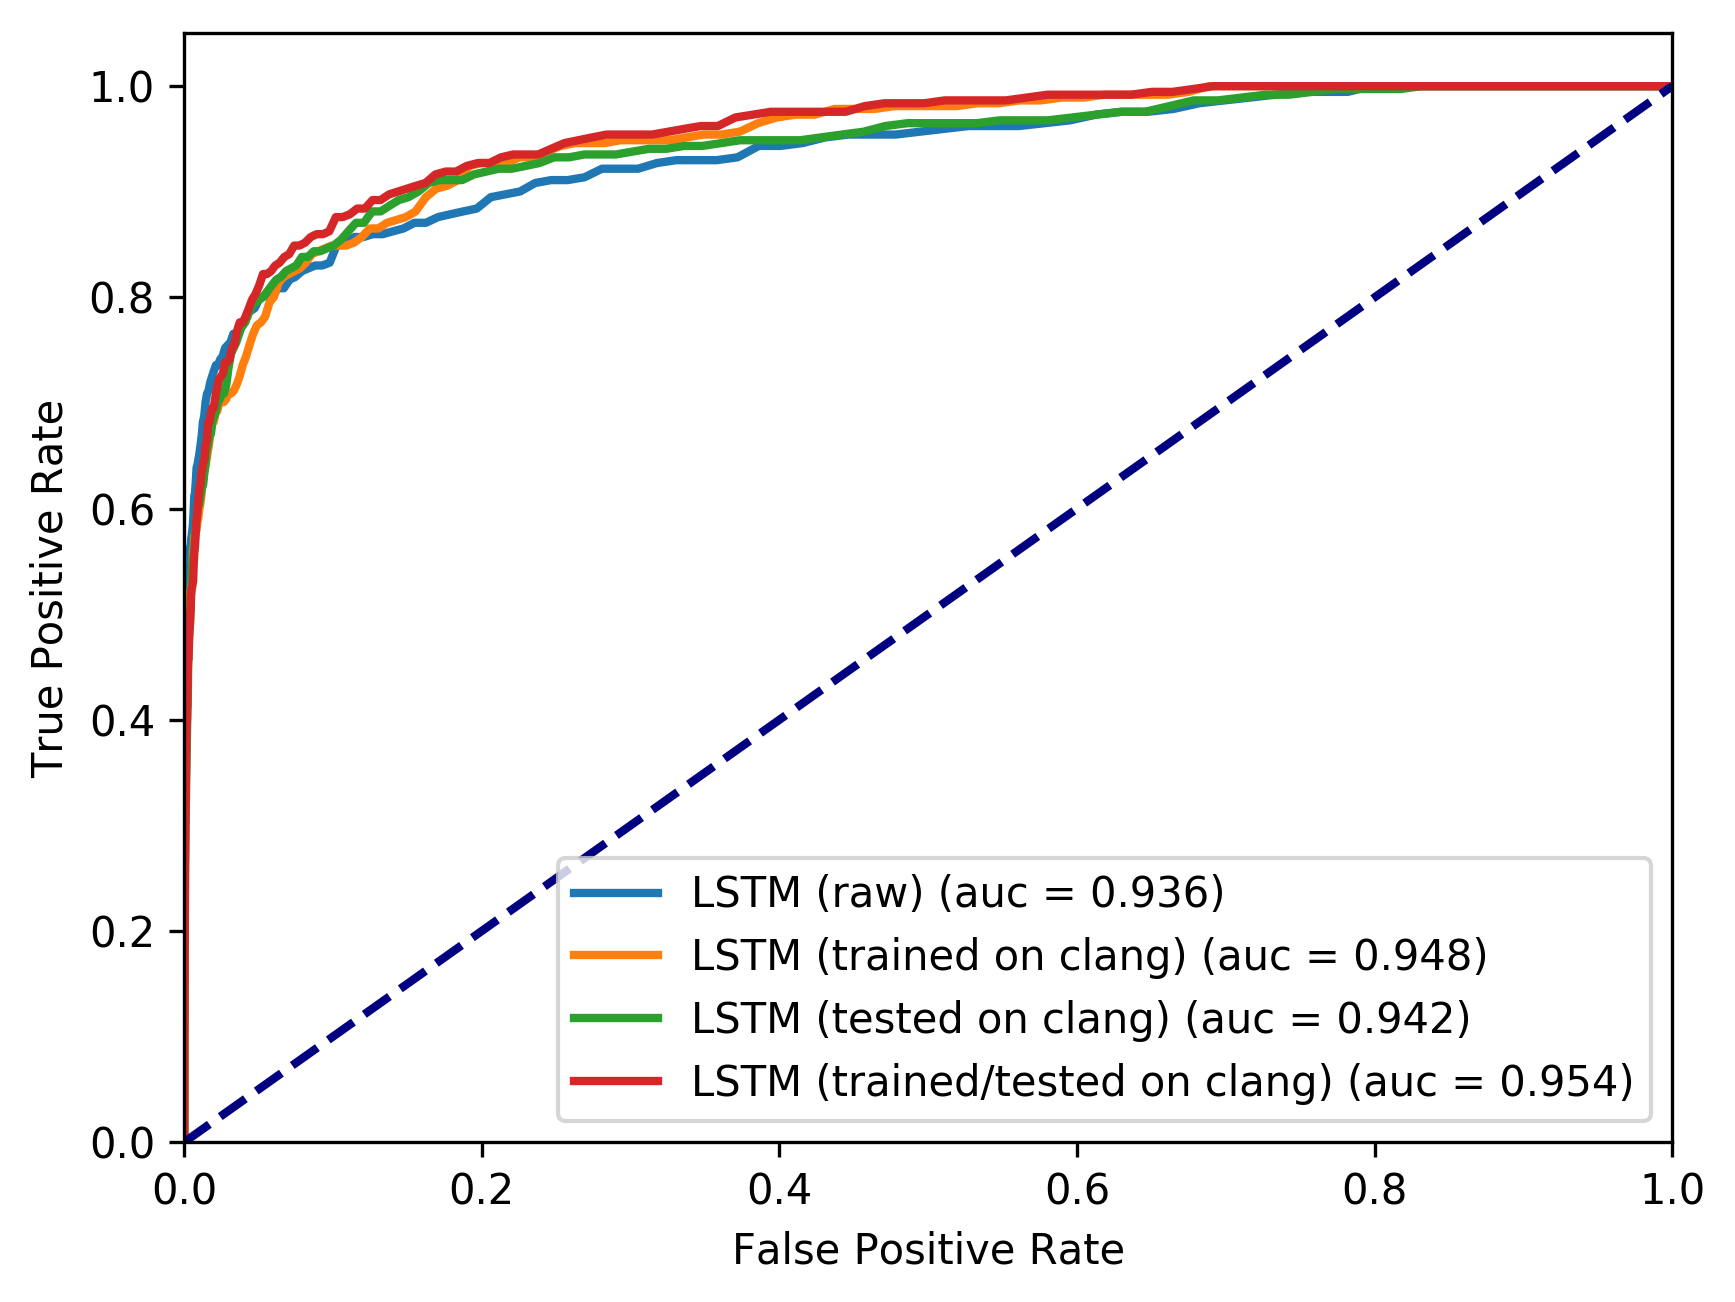
\includegraphics[width=0.7\linewidth]{imgs/roc_complete.png}
	\caption{ROC curve for each pair of classifier and dataset version.}
	\label{fig:roc_complete}
\end{figure}

Using the models we trained, we tried to solve the problem of deciding if two source codes are from the same author. For that end, we constructed a test dataset with 3,200 samples from 400 authors. These samples were extracted from the Codeforces dataset, but this set has no intersection of authors with the training and validation sets used to train the models. Therefore, the authors are unknown to the system. Moreover, we ran \textit{clang} on the samples, obtaining a \textit{clang} processed version of the test dataset.

Finally, we ran four evaluations, one for each combination of model and test dataset. The results can be seen in Fig. \ref{fig:roc_complete} and  Table \ref{tab:matching}.

\begin{table}[ht]
	\centering
	\begin{tabular}{ccr}
		\cline{2-3}
		\multicolumn{1}{l}{}                     & \multicolumn{2}{c}{\textbf{EER (\%)}}                                   \\ \cline{2-3} 
		\textbf{}                                & \textbf{Raw Test Set}     & \multicolumn{1}{l}{\textbf{\textit{clang} Test Set}} \\ \hline
		
		%\textbf{CNN (trained on raw version)}   & \multicolumn{1}{r}{16.31} & 16.88                                       \\ \hline
		%\textbf{CNN (trained on \textit{clang} version)} & \multicolumn{1}{r}{16.82} & 16.90                                        \\ \hline
		
		\textbf{LSTM (trained on raw version)}   & \multicolumn{1}{r}{13.88} & 12.24                                       \\ \hline
		\textbf{LSTM (trained on \textit{clang} version)} & \multicolumn{1}{r}{13.25} & 11.60                                        \\ \hline
	\end{tabular}
	\caption{Equal error rate (EER) evaluation of the trained models on each test set.}
	\label{tab:matching}
\end{table}

We can notice that the performance on raw source codes is slightly worse than the others. This can be related to the fact that tested authors are not present in training and validation sets. The model is probably relying more on features present on templates, instead of on stylistic features of the written code. Therefore, the embeddings generalize poorly to unknown authors. The better performance of the \textit{clang} combination supports this claim by showing that learning from features of the written code yields better generalization.

\section{One-to-Many Author Identification}\label{sec:one_to_many}

We also evaluated our models on the problem posed by \citeauthoronline{caliskan_2015}. In their work, 9 C++ source codes from 250 programmers are extracted from the Google Code Jam dataset. From these, 8 are used for training and one for testing. We simply took the models we trained for the previous experiment and replaced triplet loss with softmax cross-entropy loss. Then, we trained on the $250 \times 8$ source codes for more epochs.

The rank-$n$ metric evaluations, for $n = 1$ and $n = 3$, can be seen in Table \ref{tab:rank}.

\begin{table}[hb]
	\centering
	\begin{tabular}{lrrrr}
		\cline{2-5}
		& \multicolumn{2}{c}{\textbf{rank-1 (\%)}}                                        & \multicolumn{2}{c}{\textbf{rank-3 (\%)}}                                        \\ \cline{2-5} 
		\multicolumn{1}{c}{\textbf{}}    & \multicolumn{1}{c}{\textbf{Raw Test}} & \multicolumn{1}{l}{\textbf{Clang Test}} & \multicolumn{1}{l}{\textbf{Raw Test}} & \multicolumn{1}{l}{\textbf{Clang Test}} \\ \hline
		\textbf{LSTM (trained on raw)}   & 74.8\%                                & 67.0\%                                    & 84.4\%                                & 79.6\%                                  \\ \hline
		\textbf{LSTM (trained on clang)} & 65.0\%                                  & 69.0\%                                    & 78.8\%                                & 82.8\%                                  \\ \hline
		\textbf{\citeauthoronline{caliskan_2015}}                & 95.1\%                               & n/a                                     & n/a                                   & n/a                                     \\ \hline
	\end{tabular}
	\caption{Rank-$n$ metric for the one-to-many identification problem on 250 programmers of the Google Code Jam dataset. }
	\label{tab:rank}
\end{table}

Although we were not able to match the Random Forest model proposed by \citeauthoronline{caliskan_2015}, we are able to show that the generated descriptors are discriminative. Fig. \ref{fig:embedding} shows the style descriptors of source codes from 12 programmers of Google Code Jam dataset. They were embedded into a two-dimensional space for better visualization.

\begin{figure}[ht]
	\centering
	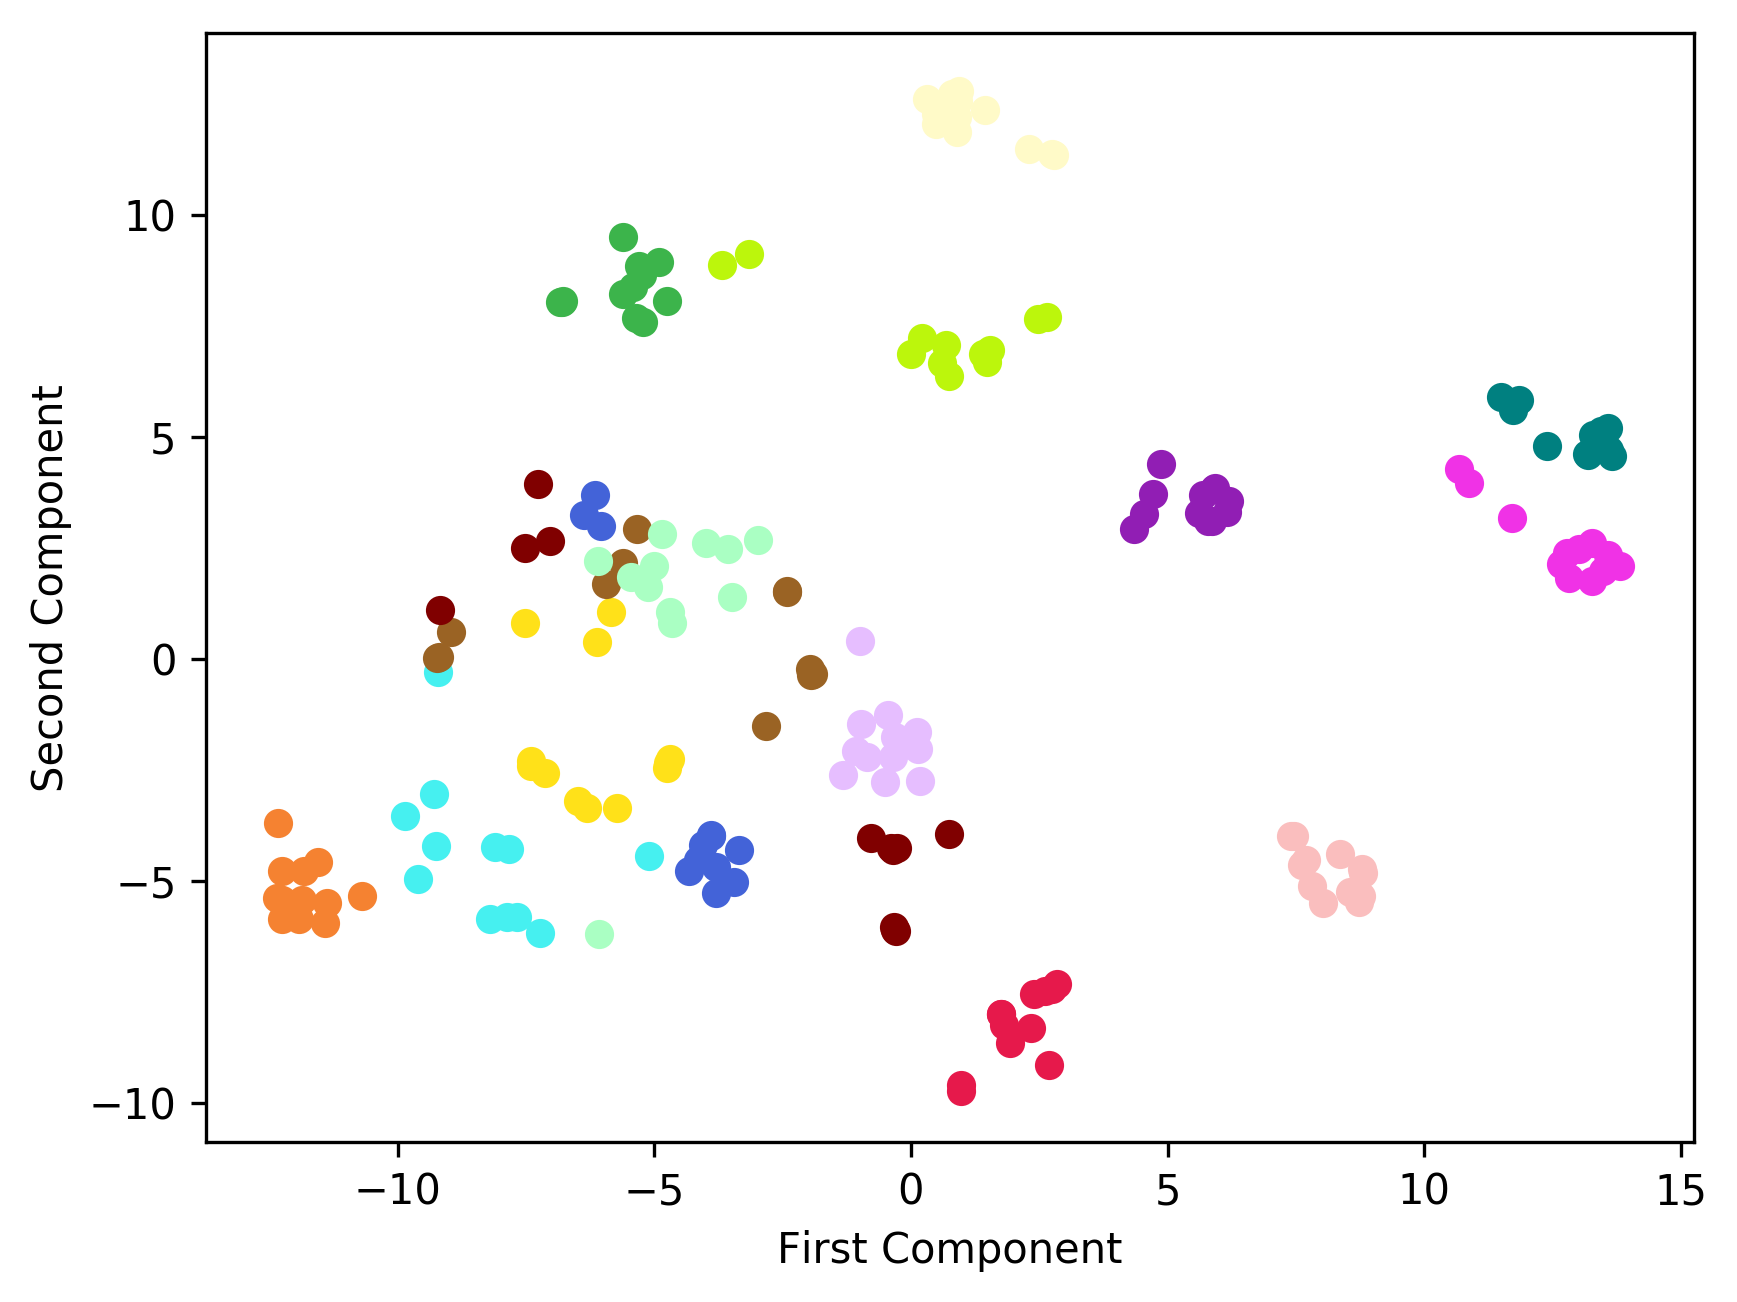
\includegraphics[width=0.7\linewidth]{imgs/embedding.png}
	\caption{128-dimensional descriptors from 12 authors generated by the LSTM model, trained and test on the \textit{clang} test set. The descriptors were embedded into a two-dimensional space with t-SNE.}
	\label{fig:embedding}
\end{figure}
\xchapter{Conclusion}{}

This work offers a study on the application of deep learning methods to the source code authorship attribution problem. In particular, we have proposed a LSTM-based model that generates descriptors which preserve stylistic similarities between source codes. Moreover, we have shown experiments supporting that stylistic features are discriminative. 

We evaluated our model in the problem of deciding if two codes were written by the same person and achieved 11.6 \% of EER. In the one-to-many identification problem, we achieved 74.8\% accuracy, 20\% less than state-of-the-art. Although we were not able to improve this result, we believe state-of-the-art deep learning methods can be successfully applied to the source code attribution problem, and that further improvements in the area will be related to that.

In the future, we hope to modify our models to support variable-length code. We also want to generate meaningful style descriptors from abstract syntax trees to improve the accuracy of our methods. Moreover, we want to be able to classify small pieces of code, like those of Git repositories.

%% Parte pos-textual
\backmatter

% Bibliografia
% É aconselhável utilizar o BibTeX a partir de um arquivo, digamos "biblio.bib".
% Para ajuda na criação do arquivo .bib e utilização do BibTeX, recorra ao
% BibTeXpress em www.cin.ufpe.br/~paguso/bibtexpress
\bibliographystyle{abntex2-alf}
\bibliography{src/biblio}

% Apendices
% Comente se naoo houver apendices
\iffalse
\appendix

\xchapter{Exemplo de Apêndice}{} %sem preambulo
\lipsum
\fi
% Eh aconselhavel criar cada apendice em um arquivo separado, digamos
% "apendice1.tex", "apendice.tex", ... "apendiceM.tex" e depois
% inclui--los com:
% \include{apendice1}
% \include{apendice2}
% ...
% \include{apendiceM}

%% Fim do documento
\end{document}
%------------------------------------------------------------------------------------------%